\documentclass[11pt,a4paper]{article}

\usepackage[T1]{fontenc}
\usepackage[utf8]{inputenc}
\usepackage{lmodern}
\usepackage[spanish,es-tabla,es-noshorthands,es-nodecimaldot]{babel}
\usepackage[a4paper,margin=2.5cm]{geometry}
\usepackage{microtype}
\usepackage{amsmath,amssymb}
\usepackage{booktabs,tabularx,multirow,makecell}
\usepackage{graphicx}
\usepackage[font=small,labelfont=bf,skip=4pt]{caption}
\usepackage[round,authoryear]{natbib}
\usepackage{xcolor}
\usepackage[colorlinks=true,linkcolor={blue!50!black},citecolor={blue!50!black},urlcolor={blue!50!black}]{hyperref}
\usepackage{enumitem}
\usepackage{xurl}
\usepackage[section]{placeins}
\setlist{itemsep=2pt,topsep=4pt}
\graphicspath{{../figures/es/}}
\setlength{\parskip}{3pt}
\renewcommand{\arraystretch}{1.12}
\renewcommand{\topfraction}{0.85}
\renewcommand{\bottomfraction}{0.6}
\renewcommand{\textfraction}{0.12}
\renewcommand{\floatpagefraction}{0.8}
\setcounter{topnumber}{3}
\setcounter{totalnumber}{4}

\hypersetup{pdftitle={La prima de riesgo de varianza del S\&P 500},pdfauthor={Borja Izquierdo Piñero},pdfkeywords={VRP, variance risk premium, gradient boosting, purged cross-validation}}
\newcommand{\repourl}{\url{https://github.com/borja-izquierdo/vrp-sp500-options}}
\newcommand{\E}{\mathbb{E}}

\title{\textbf{La prima de riesgo de varianza del S\&P~500:\\
predicción con \textit{gradient boosting} y valor económico de la señal}\\[4pt]
\large Versión revisada y ampliada de un Trabajo Fin de Máster}
\author{Borja Izquierdo Piñero}
\date{Octubre de 2026}

\begin{document}
\maketitle

\begin{abstract}
\noindent
Este trabajo estudia si un modelo de \textit{gradient boosting} que predice la prima de riesgo de varianza (VRP) del S\&P~500 mejora una estrategia de venta de volatilidad cubierta en delta, una vez descontados los costes y evaluada fuera de muestra. Con opciones mensuales sobre el SPX y datos de 2018 a 2025, la prima es persistente: la volatilidad implícita superó a la realizada en el 87,4~\% de las sesiones. Un modelo XGBoost con 22 predictores y validación cruzada purgada reduce el error cuadrático medio un 6~\% frente a la media histórica, aunque la mejora no es significativa con el contraste de Diebold y Mariano. En la capa de operación, la señal no aporta valor. Todas las predicciones fuera de muestra son positivas, por lo que la estrategia guiada por el modelo coincide con la venta incondicional, y la predicción no ordena el resultado de las operaciones. La ventaja frente a una regla ingenua que se atribuyó en la versión original del trabajo no procede del modelo, sino de que la comparación no era homogénea. El resultado económico depende sobre todo de la calibración de la cobertura y del tratamiento del colateral. Con colateral remunerado, venta al precio comprador y la banda de cobertura de la versión original, la venta sistemática obtiene un Sharpe de 0,23, pero esa banda se eligió dentro de la muestra y su óptimo no es estable fuera de ella. Un swap de varianza sintético confirma estas conclusiones en un marco libre de supuestos de ejecución y cuantifica la pérdida de febrero de 2018 en unos veinte meses de prima media. Ninguna diferencia entre estrategias es estadísticamente significativa.

\medskip
\noindent\textbf{Palabras clave:} prima de riesgo de varianza, volatilidad implícita, \textit{gradient boosting}, validación cruzada purgada, cobertura delta, swaps de varianza.\\
\textbf{Clasificación JEL:} C53, G13, G17.
\end{abstract}

\vspace{-2pt}
\noindent\fcolorbox{gray!50}{gray!6}{\parbox{\dimexpr\linewidth-2\fboxsep-2\fboxrule}{\small
\textbf{Nota sobre esta versión.} Este documento revisa el Trabajo Fin de Máster \textit{Arbitraje estadístico de volatilidad: modelado del Variance Risk Premium mediante Machine Learning} (Máster en Asesoramiento y Planificación Financiera, Universidad Rey Juan Carlos, julio de 2026). Corrige la interpretación de la comparación entre la estrategia predictiva y la regla sistemática (sección~\ref{sec:correccion}) y añade validación anidada, referencias ingenuas, contrastes estadísticos, costes de ejecución, remuneración del colateral y un análisis con swaps de varianza sintéticos (secciones~\ref{sec:prediccion} a \ref{sec:inferencia}). El código y los resultados son reproducibles en \repourl.}}

\section{Introducción}\label{sec:intro}

La volatilidad implícita en los precios de las opciones sobre índices bursátiles tiende a superar la volatilidad que el índice realiza después. Esa diferencia, la prima de riesgo de varianza o \textit{variance risk premium} (VRP), es una de las regularidades mejor documentadas de los mercados de derivados \citep{carrwu2009} y remunera a quien vende volatilidad. Su captura tiene, sin embargo, un perfil de riesgo muy asimétrico: ganancias pequeñas y frecuentes frente a pérdidas raras pero de gran magnitud. El 5 de febrero de 2018 el VIX pasó de 18,44 a 37,32 en una sola sesión, y los productos cotizados inversos sobre el VIX perdieron cerca del 97~\% de su valor antes de la apertura siguiente \citep{augustin2021}. El 21 de febrero Credit Suisse anunció la amortización anticipada del XIV a 5,99 dólares por título \citep{varadarajan2023}.

La pregunta de este trabajo es si un modelo de aprendizaje automático que predice la prima permite venderla de forma más eficiente que una regla mecánica, es decir, si mejora la relación entre rentabilidad y riesgo de una estrategia de venta de volatilidad cubierta en delta, neta de costes y fuera de muestra. Para responderla se construye un sistema completo: descarga y depuración de cadenas de opciones del SPX, 22 predictores, modelos XGBoost y LightGBM con pérdida de Huber y validación cruzada purgada, y un motor de simulación histórica que vende \textit{straddles} sobre el SPX y los cubre en delta con comisiones y deslizamiento.

Las aportaciones son cuatro. En primer lugar, el sistema es reproducible de extremo a extremo con datos que cualquier investigador puede adquirir. En segundo lugar, la capacidad predictiva se evalúa frente a referencias ingenuas con el contraste de \citet{dieboldmariano1995}, y no solo en términos absolutos. En tercer lugar, se separa la calidad de la predicción de su valor económico: se mide si la predicción ordena el resultado de las operaciones, si su magnitud mejora la entrada o el tamaño de la posición y qué parte del resultado procede de los costes, del colateral y de la cobertura. Por último, la prima se mide también con swaps de varianza sintéticos, lo que permite cubrir todo el periodo, incluido el año 2021, para el que no se dispone de cadenas de opciones, y cuantificar la pérdida de febrero de 2018.

Los resultados son mixtos y se presentan sin matices defensivos:
\begin{itemize}
  \item La prima existe y es persistente: positiva en el 87,4~\% de las sesiones, con una media de 4,95 puntos de volatilidad.
  \item El modelo predice mejor que las referencias ingenuas en promedio, pero no en todos los periodos, y la mejora en error cuadrático no es significativa.
  \item La señal no llega a la capa de operación. Todas las predicciones del modelo seleccionado son positivas, de modo que la estrategia predictiva equivale a vender siempre. Su correlación de rangos con el resultado de cada operación es de 0,05.
  \item La comparación con la regla sistemática del trabajo original no era homogénea: el recuento de operaciones de la regla incluía un periodo anterior a la ventana de evaluación. En términos homogéneos, no hay ventaja atribuible al modelo.
  \item Lo que determina el resultado es la gestión del riesgo: la amplitud de la banda de cobertura y, en menor medida, la remuneración del colateral. Ninguna de las diferencias entre estrategias es estadísticamente significativa con 6,7 años y 64 operaciones.
\end{itemize}

El resto del documento se organiza así. La sección~\ref{sec:marco} resume el marco conceptual. La sección~\ref{sec:datos} describe los datos y la sección~\ref{sec:metodo}, la metodología. La sección~\ref{sec:resultados} presenta los resultados, la sección~\ref{sec:limitaciones} discute las limitaciones y las extensiones, y la sección~\ref{sec:conclusiones} concluye.

\section{Marco conceptual}\label{sec:marco}

\subsection{La prima de riesgo de varianza}

Un swap de varianza es un contrato a plazo sobre la varianza realizada. Al vencimiento, el comprador recibe $N_{\text{var}}\,(RV_{t,T}-K^2)$, donde $RV_{t,T}$ es la varianza anualizada de los rendimientos diarios entre $t$ y $T$, y $K^2$ es el precio de ejercicio pactado. Como la entrada no tiene coste, $K^2$ es la esperanza de la varianza realizada bajo la medida neutral al riesgo $\mathbb{Q}$, y \citet{carrwu2009} muestran que puede replicarse con una cartera estática de opciones fuera de dinero. La prima de riesgo de varianza es la diferencia entre la expectativa neutral al riesgo y la expectativa física $\mathbb{P}$:
\begin{equation}
  \text{VRP}_t = \E^{\mathbb{Q}}_t[RV_{t,T}] - \E^{\mathbb{P}}_t[RV_{t,T}].
\end{equation}
Para los índices bursátiles esta diferencia es positiva y elevada desde el punto de vista del vendedor de varianza \citep{carrwu2009}. Su origen es un desequilibrio estructural entre la demanda de protección, concentrada en opciones de venta fuera de dinero, y la oferta de quienes asumen el riesgo de cola. Los creadores de mercado que actúan como contrapartida quedan cortos de gamma, por lo que exigen una compensación por las pérdidas que sufren ante saltos discontinuos del precio \citep{ang2018,israelov2019}.

La volatilidad implícita libre de modelo (MFIV) es la raíz cuadrada del precio de ejercicio del swap de varianza a 30 días. La metodología del VIX la calcula a partir de las opciones fuera de dinero de los dos vencimientos que rodean los 30 días \citep{cboe2019}:
\begin{equation}\label{eq:mfiv}
  \sigma^2_{\text{MFIV}} = \frac{2}{T}\sum_i \frac{\Delta K_i}{K_i^2}\,e^{rT}\,Q(K_i) - \frac{1}{T}\left(\frac{F}{K_0}-1\right)^2,
\end{equation}
donde $Q(K_i)$ es el precio medio de la opción fuera de dinero de precio de ejercicio $K_i$, $F$ el nivel a plazo del índice y $K_0$ el primer precio de ejercicio inferior a $F$. El VIX dividido por 100 es, por construcción, la MFIV a 30 días del S\&P~500, y así se utiliza en este trabajo.

\subsection{Venta de volatilidad cubierta en delta}

Un \textit{straddle} vendido (venta de una opción de compra y una de venta con el mismo precio de ejercicio y vencimiento) nace con delta próxima a cero y gamma negativa. Si la posición se cubre continuamente en delta, su resultado diario es aproximadamente
\begin{equation}\label{eq:gamma}
  d\Pi_t \approx \tfrac{1}{2}\,\Gamma_t S_t^2\left(\sigma^2_{\text{imp}}-\sigma^2_{\text{real},t}\right)dt,
\end{equation}
con $\Gamma_t<0$ para la posición vendida \citep{sinclair2008}. El vendedor gana cuando la volatilidad realizada queda por debajo de la implícita y pierde en caso contrario, con una pérdida que crece de forma convexa con la magnitud del movimiento. Los índices de venta sistemática de opciones reflejan este perfil: entre 1986 y 2018 el índice CBOE PutWrite tuvo una volatilidad del 9,9~\% frente al 14,9~\% del S\&P~500, pero con una asimetría de $-2{,}10$ y una curtosis de 9,72 \citep{wilshire2019}.

En la práctica, la cobertura es discreta. Rebalancear con frecuencia reduce el riesgo de gamma pero multiplica los costes; rebalancear poco ahorra costes pero deja expuesta la posición. La banda de tolerancia de la cobertura es, por tanto, un parámetro económico de primer orden, como confirma la sección~\ref{sec:costes}.

\subsection{Aprendizaje automático y validación temporal}

Los modelos de \textit{gradient boosting} aproximan la función objetivo mediante una suma de árboles de regresión ajustados secuencialmente a los pseudorresiduos del conjunto anterior \citep{friedman2001}. XGBoost utiliza una aproximación de segundo orden de la pérdida y regularización L1 y L2 sobre los pesos de las hojas \citep{chen2016}; LightGBM hace crecer los árboles por hojas y emplea muestreo basado en gradientes \citep{ke2017}. Frente a los modelos lineales y la familia GARCH \citep{bollerslev1986}, capturan relaciones no lineales e interacciones sin especificarlas de antemano, una ventaja documentada en problemas de predicción con muchos predictores \citep{medeiros2021}.

En series financieras, la validación cruzada aleatoria introduce sesgo de anticipación. Cuando la variable objetivo se construye con información futura, como ocurre aquí con la volatilidad de las 21 sesiones siguientes, además hay solapamiento entre las etiquetas de entrenamiento y las de prueba. \citet{lopezdeprado2018} propone purgar las observaciones de entrenamiento cuyas etiquetas se solapan con el bloque de prueba y añadir un periodo de embargo.

\section{Datos}\label{sec:datos}

\begin{table}[!htbp]
\centering
\caption{Fuentes de datos}\label{tab:datos}
\small
\begin{tabularx}{\linewidth}{@{}>{\raggedright\arraybackslash}p{3.3cm}X>{\raggedright\arraybackslash}p{4.4cm}@{}}
\toprule
Fuente & Series & Uso \\
\midrule
ThetaData (plan Options Standard) & Opciones mensuales del SPX (tercer viernes): cotizaciones de cierre, griegas, volatilidad implícita e interés abierto & Predictores, selección y valoración de las posiciones \\
Stooq (yfinance como alternativa) & Precios diarios de apertura, máximo, mínimo y cierre del SPX & Volatilidad realizada, cobertura, Buy \& Hold \\
FRED & VIXCLS, DGS3MO, DGS10 & MFIV, tipos, pendiente, colateral \\
yfinance & Índice CBOE SKEW & Predictor de riesgo de cola \\
\bottomrule
\end{tabularx}
\end{table}

La muestra abarca del 2 de enero de 2018 al 31 de diciembre de 2025: 2.011 sesiones y 96 vencimientos mensuales (tabla~\ref{tab:datos}). Se emplean opciones sobre el SPX y no sobre el SPY porque son de estilo europeo, se liquidan por diferencias y constituyen el mercado de volatilidad más profundo, sobre el que se calcula el propio VIX \citep{cboe2019}.

La cadena se depura con cinco filtros: volumen positivo e interés abierto de al menos 100 contratos; cotizaciones válidas ($0<\text{bid}<\text{ask}$); diferencial relativo no superior al 20~\% del precio medio; vencimiento entre 15 y 45 días; y \textit{moneyness} ($K/S$) entre 0,85 y 1,15. Tras la depuración quedan 341.094 observaciones, en torno al 7--9~\% de la cadena original.

Las cadenas de 2021 no pudieron recuperarse por una incidencia en la descarga. Ese año el modelo dispone de las variables de mercado y de volatilidad realizada, pero no de las microestructurales, y la estrategia con opciones no opera. El análisis con swaps de varianza (sección~\ref{sec:varswap}) no depende de las opciones y sí cubre 2021.

\section{Metodología}\label{sec:metodo}

\subsection{Variable objetivo}

La variable objetivo es la prima de volatilidad realizada a 21 sesiones:
\begin{equation}\label{eq:target}
  y_t = \sigma_{\text{MFIV},t} - \sigma^{\text{YZ}}_{(t,\,t+21]},
\end{equation}
donde $\sigma_{\text{MFIV},t}$ es el VIX dividido por 100 y $\sigma^{\text{YZ}}$ es el estimador de \citet{yangzhang2000} sobre las 21 sesiones siguientes. Este estimador combina el salto nocturno, la variación entre apertura y cierre y el término de Rogers-Satchell, y es insesgado en presencia de deriva y de saltos de apertura. La prima se expresa en volatilidad: 0,05 equivale a 5 puntos de volatilidad.

\subsection{Predictores}

Los 22 predictores (tabla~\ref{tab:features}) solo utilizan información disponible al cierre de la sesión $t$ y se agrupan en tres familias: volatilidad realizada en ventanas de 21 sesiones, con los estimadores de cierre a cierre, \citet{parkinson1980}, \citet{garmanklass1980} y Yang-Zhang; microestructura del mercado de opciones, medida sobre el vencimiento más próximo a 30 días; y variables de mercado y momento.

\begin{table}[!htbp]
\centering
\caption{Predictores}\label{tab:features}
\small
\begin{tabularx}{\linewidth}{@{}lX@{}}
\toprule
Familia & Variables \\
\midrule
Volatilidad realizada (21 sesiones) & \texttt{rv\_cc}, \texttt{rv\_parkinson}, \texttt{rv\_gk}, \texttt{rv\_yz} \\
Microestructura de opciones & \texttt{atm\_iv}; \texttt{skew\_slope} (VI de la put de delta $-0{,}25$ menos VI de la call de delta $0{,}25$); \texttt{pcr\_volume}, \texttt{pcr\_oi}; \texttt{iv\_rank}, \texttt{iv\_percentile} (252 sesiones) \\
Mercado y momento & \texttt{mfiv}, \texttt{vix}, \texttt{vix\_chg}, \texttt{skew}, \texttt{skew\_chg}, \texttt{ust\_3m}, \texttt{ust\_10y}, \texttt{term\_slope}; \texttt{ret\_5d}, \texttt{ret\_10d}, \texttt{ret\_21d}, \texttt{ret\_63d} \\
\bottomrule
\end{tabularx}
\end{table}

\subsection{Modelos y validación}

Se comparan XGBoost y LightGBM con una pérdida de Huber \citep{huber1964} de umbral $\delta=0{,}02$, que se comporta de forma cuadrática para errores pequeños y lineal para los grandes, y limita así la influencia de episodios extremos como marzo de 2020. Los hiperparámetros se eligen por búsqueda aleatoria de 40 combinaciones sobre una malla (apéndice~\ref{app:hiper}), con semilla fija.

La validación es temporal y de ventana creciente, con cinco pliegues. Entre el final de cada bloque de entrenamiento y el inicio del bloque de prueba se eliminan $21+5$ sesiones: 21 de purga, la longitud de la etiqueta, y 5 de embargo. En la versión original del trabajo, la búsqueda de hiperparámetros y la elección entre XGBoost y LightGBM se evaluaban sobre los mismos pliegues que después se informan. Esta revisión añade una \textbf{validación anidada}: para cada pliegue externo, ambos modelos realizan su búsqueda en una validación purgada interna de tres pliegues dentro del bloque de entrenamiento, y el modelo y los parámetros con menor pérdida interna se reestiman sobre todo el bloque y predicen el bloque de prueba. Ninguna decisión que se evalúa en un bloque utiliza información de ese bloque.

\subsection{Referencias ingenuas y contraste de capacidad predictiva}

El modelo se compara con dos predicciones sin aprendizaje, evaluadas en los mismos pliegues: la media de la variable objetivo en el bloque de entrenamiento, y la prima ingenua $\sigma_{\text{MFIV},t}-\sigma^{\text{YZ}}_{(t-21,\,t]}$, que supone que la volatilidad realizada se mantendrá en su nivel reciente. La igualdad de capacidad predictiva se contrasta con el estadístico de \citet{dieboldmariano1995}, con varianza de largo plazo de \citet{neweywest1987} con 20 retardos (por el solapamiento de las etiquetas de 21 sesiones) y la corrección de muestras finitas de \citet{hln1997}.

\subsection{Estrategia con opciones}\label{sec:estrategia}

La estrategia es la de la versión original. Cuando no hay posición abierta y la señal de la sesión supera el umbral, se vende un \textit{straddle} en el dinero sobre el vencimiento más próximo a 30 días. La posición se valora a diario con los precios medios de la cadena y se cubre con el índice cuando la delta neta, en valor absoluto, supera la banda $b\times$ contratos $\times$ multiplicador. Cada operación de cobertura paga 1 punto básico de deslizamiento y cada opción, 1 dólar de comisión, y la posición se liquida al vencimiento por su valor intrínseco. Cuando una opción no tiene cotización, lo que ocurre sistemáticamente en los últimos 15 días por el filtro de vencimiento, se valora con Black-Scholes \citep{blackscholes1973,merton1973} y la última volatilidad implícita observada. El tamaño es de un contrato sobre un capital de un millón de dólares; con el SPX en 2.943 puntos al inicio de la ventana, cada pata equivale a unos 294.000 dólares de nocional.

La ventana de evaluación va del 29 de abril de 2019, primera predicción fuera de muestra, al 31 de diciembre de 2025. Sobre esta base se definen dos configuraciones:
\begin{itemize}
  \item \textbf{Configuración de la tesis}: entrada al precio medio, colateral sin remunerar, ratio de Sharpe con un tipo libre de riesgo fijo del 2~\% y banda $b=0{,}50$, elegida en el trabajo original por su resultado en la misma muestra.
  \item \textbf{Configuración rigurosa}: venta al precio comprador (\textit{bid}), colateral remunerado al día con el rendimiento de la letra del Tesoro a tres meses (DGS3MO), Sharpe calculado sobre el exceso frente a ese mismo tipo, predicciones de la validación anidada y banda elegida en cada pliegue. La banda es la que maximiza el Sharpe de la venta incondicional en los datos anteriores al bloque de prueba.
\end{itemize}
Para medir el valor de la magnitud de la predicción, y no solo de su signo, se comparan cinco señales: vender siempre; ML $>0$ (regla original); ML $>$ mediana, que solo vende cuando la prima prevista supera la mediana de la prima realizada en el bloque de entrenamiento; ML con tamaño, que vende $\min(\max(\hat y_t/m,0),3)$ contratos, con $m$ esa misma mediana; e ingenua $>$ mediana, que aplica el mismo umbral a la prima ingenua. Todos los umbrales se fijan con información del bloque de entrenamiento.

\subsection{Swaps de varianza sintéticos}\label{sec:metodo_vs}

Para medir la prima sin depender del motor de opciones se simula la venta de swaps de varianza a 21 sesiones con precio de ejercicio $K=\text{VIX}_t$ (en puntos de volatilidad). El resultado por unidad de nocional vega es
\begin{equation}\label{eq:vswap}
  \pi_t = \frac{K_t^2 - RV_{(t,\,t+21]}}{2K_t},
  \qquad RV_{(t,\,t+21]} = \frac{252}{21}\sum_{i=1}^{21} r_{t+i}^2 \times 10^4,
\end{equation}
con $r$ los rendimientos logarítmicos diarios del SPX. Un swap con 100.000 dólares de nocional vega gana o pierde 100.000 dólares por cada punto de $\pi_t$. La estrategia vende un swap cada 21 sesiones, sin solapamiento, y los estadísticos se promedian sobre los 21 calendarios de entrada posibles. Como robustez se aplica el límite habitual de la volatilidad realizada a 2,5 veces el precio de ejercicio. El análisis ignora que los swaps cotizan algo por encima del VIX al cuadrado, por convexidad y saltos.

\subsection{Inferencia sobre las estrategias}

Los intervalos de confianza del ratio de Sharpe y de las diferencias de Sharpe entre estrategias se obtienen con el \textit{bootstrap} estacionario de \citet{politisromano1994}, con bloques de longitud media de 21 sesiones y 10.000 remuestreos. Las dos series de cada comparación se remuestrean con los mismos bloques, en la línea de \citet{ledoitwolf2008}.

\section{Resultados}\label{sec:resultados}

\subsection{La prima: hechos estilizados}

La figura~\ref{fig:vrp} muestra la volatilidad implícita y la realizada en las 21 sesiones siguientes. La prima de la ecuación~\eqref{eq:target} es positiva en el 87,4~\% de las sesiones, con una media de 0,0495 y una desviación típica de 0,0724. Su distribución tiene una cola izquierda pronunciada: la prima se vuelve muy negativa cuando la volatilidad realizada se acelera más deprisa que la implícita, como en enero y febrero de 2018 o en febrero y marzo de 2020, con un mínimo de $-0{,}486$.

\begin{figure}[!htbp]
\centering
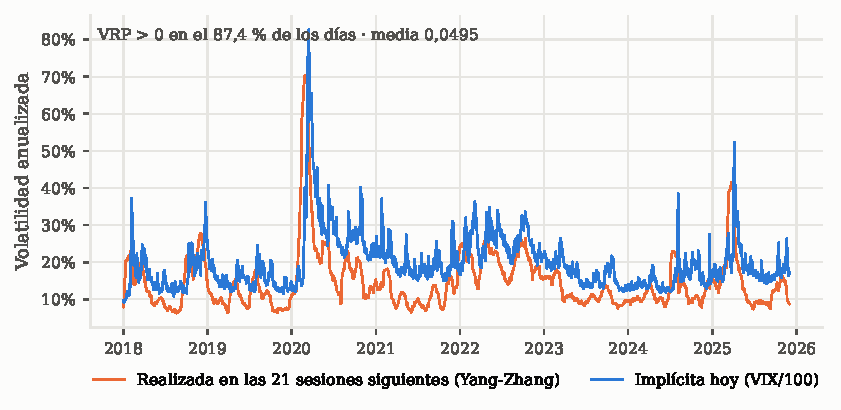
\includegraphics[width=\linewidth]{fig01_vrp_series.pdf}
\caption{Volatilidad implícita (VIX/100) y volatilidad realizada en las 21 sesiones siguientes (Yang-Zhang), 2018--2025.}\label{fig:vrp}
\end{figure}

La tabla~\ref{tab:vs_year} y la figura~\ref{fig:vs_year} presentan la misma prima en forma de swap de varianza vendido cada sesión. Los años de crisis (2018 y 2020) tienen resultado medio negativo, y 2021 es el mejor año de la muestra: el swap vendido ganó una media de 5,4 puntos de volatilidad y fue rentable el 95~\% de los días. Que la estrategia con opciones no opere en 2021 por falta de datos la penaliza.

\begin{table}[!htbp]
\centering
\caption{Swap de varianza vendido a 21 sesiones, entrada diaria (puntos de volatilidad por unidad de nocional vega)}\label{tab:vs_year}
\small
\begin{tabular}{@{}lrrrrr@{}}
\toprule
Año & $K$ medio & $\sqrt{RV}$ medio & P\&L medio & \% días positivos & Peor día \\
\midrule
2018 & 16,6 & 15,9 & $-1{,}0$ & 61 & $-25{,}1$ \\
2019 & 15,4 & 11,2 & 3,1 & 84 & $-15{,}1$ \\
2020 & 29,3 & 27,1 & $-7{,}3$ & 77 & $-252{,}2$ \\
2021 & 19,7 & 12,8 & 5,4 & 95 & $-2{,}2$ \\
2022 & 25,6 & 23,7 & 1,3 & 65 & $-19{,}8$ \\
2023 & 16,9 & 12,6 & 3,7 & 100 & 0,1 \\
2024 & 15,6 & 12,4 & 2,4 & 81 & $-11{,}2$ \\
2025 & 19,3 & 16,0 & 0,8 & 83 & $-59{,}3$ \\
\bottomrule
\end{tabular}
\end{table}

\begin{figure}[!htbp]
\centering
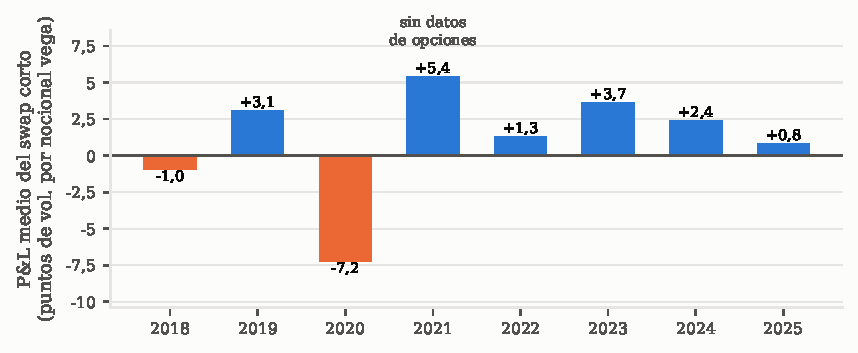
\includegraphics[width=\linewidth]{fig02_varswap_by_year.pdf}
\caption{Resultado medio anual del swap de varianza vendido a 21 sesiones con entrada diaria. 2021, el año sin cadenas de opciones, es el más favorable para el vendedor.}\label{fig:vs_year}
\end{figure}

\subsection{Capacidad predictiva}\label{sec:prediccion}

La tabla~\ref{tab:forecast} recoge las métricas fuera de muestra. XGBoost, el modelo seleccionado en la versión original, obtiene un RMSE medio de 0,0662, un 6~\% inferior al de la media de entrenamiento (0,0704) y un 14~\% inferior al de la prima ingenua (0,0766). La mejora no es uniforme: el modelo pierde frente a la media de entrenamiento en los pliegues 3 y 5 (figura~\ref{fig:folds}). Con validación anidada, que en el primer pliegue selecciona LightGBM, el RMSE medio sube a 0,0675 y la correlación baja de 0,21 a 0,16. Parte de la ventaja original procedía, por tanto, de elegir los hiperparámetros con los mismos datos de evaluación.

\begin{table}[!htbp]
\centering
\caption{Capacidad predictiva fuera de muestra: RMSE por pliegue y medias}\label{tab:forecast}
\footnotesize\setlength{\tabcolsep}{4.2pt}
\begin{tabular}{@{}lccccc|cccc@{}}
\toprule
& \multicolumn{5}{c|}{RMSE por pliegue} & \multicolumn{4}{c}{Media de los pliegues} \\
Predicción & 1 & 2 & 3 & 4 & 5 & RMSE & MAE & Corr. & Acierto dir. \\
\midrule
XGBoost (tesis) & 0,1289 & 0,0437 & 0,0510 & 0,0356 & 0,0718 & 0,0662 & 0,0426 & 0,212 & 0,905 \\
Anidada & 0,1329 & 0,0468 & 0,0506 & 0,0359 & 0,0716 & 0,0675 & 0,0473 & 0,156 & 0,898 \\
Media de entrenamiento & 0,1295 & 0,0680 & 0,0463 & 0,0386 & 0,0698 & 0,0704 & 0,0491 & -- & 0,905 \\
Ingenua & 0,1581 & 0,0490 & 0,0539 & 0,0371 & 0,0848 & 0,0766 & 0,0512 & 0,110 & 0,848 \\
\bottomrule
\end{tabular}
\par\smallskip\raggedright\footnotesize Pliegues de prueba: abr.\,2019--ago.\,2020, ago.\,2020--dic.\,2021, dic.\,2021--abr.\,2023, abr.\,2023--jul.\,2024 y ago.\,2024--dic.\,2025.
\end{table}

\begin{figure}[!htbp]
\centering
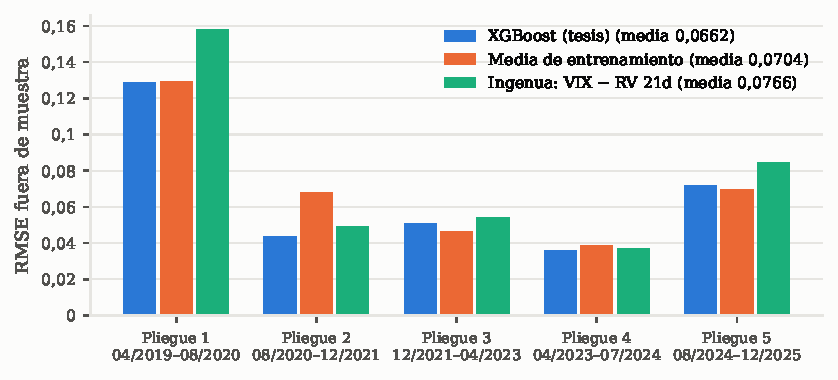
\includegraphics[width=\linewidth]{fig03_forecast_folds.pdf}
\caption{RMSE fuera de muestra por pliegue de la validación purgada: XGBoost frente a la media de entrenamiento y a la prima ingenua.}\label{fig:folds}
\end{figure}

El acierto direccional del 90,5~\% que destacaba la versión original no tiene contenido informativo. Coincide con el de una predicción constante positiva, porque la prima fue positiva en el 90~\% de los días de prueba, y la figura~\ref{fig:pred} muestra el motivo: la predicción de XGBoost oscila entre 0,021 y 0,181 y no es negativa en ninguna de las 1.659 sesiones. La pérdida de Huber y la preponderancia de primas positivas en el entrenamiento llevan al modelo a predecir el nivel típico de la prima y a no anticipar sus caídas.

\begin{figure}[!htbp]
\centering
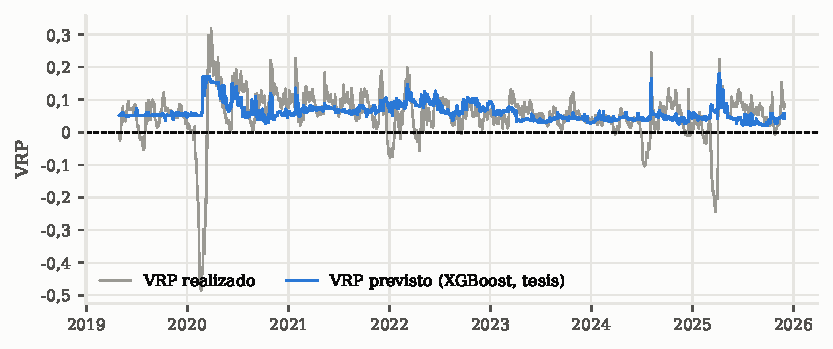
\includegraphics[width=\linewidth]{fig04_prediction_vs_target.pdf}
\caption{Prima prevista por XGBoost (tesis) y prima realizada. La predicción no cruza nunca el cero.}\label{fig:pred}
\end{figure}

La tabla~\ref{tab:dm} contrasta formalmente la diferencia. En error cuadrático, la mejora de XGBoost frente a la media de entrenamiento no es significativa ($p=0{,}27$); en error absoluto sí lo es ($p=0{,}009$), lo que indica que el modelo acierta mejor en los días normales sin mejorar en los extremos, que dominan el error cuadrático. Frente a la prima ingenua la evidencia es débil ($p$ entre 0,03 y 0,06). Con validación anidada ninguna mejora es significativa al 5~\%.

\begin{table}[!htbp]
\centering
\caption{Contraste de Diebold-Mariano (H$_1$: el modelo es más preciso). Estadístico con corrección HLN y $p$-valor unilateral; $n=1.659$}\label{tab:dm}
\small
\begin{tabular}{@{}llcccc@{}}
\toprule
& & \multicolumn{2}{c}{Error cuadrático} & \multicolumn{2}{c}{Error absoluto} \\
Modelo & Referencia & DM & $p$ & DM & $p$ \\
\midrule
XGBoost (tesis) & Media de entrenamiento & $-0{,}61$ & 0,272 & $-2{,}37$ & 0,009 \\
XGBoost (tesis) & Ingenua & $-1{,}52$ & 0,064 & $-1{,}91$ & 0,028 \\
Anidada & Media de entrenamiento & $-0{,}87$ & 0,192 & $-1{,}05$ & 0,147 \\
Anidada & Ingenua & $-1{,}63$ & 0,052 & $-1{,}12$ & 0,132 \\
\bottomrule
\end{tabular}
\end{table}

La importancia de las variables del modelo de la tesis, reestimado sobre toda la muestra, se concentra en el nivel de la volatilidad implícita (\texttt{mfiv} 0,126 y \texttt{vix} 0,123), seguido de los tipos a tres meses y a diez años (0,079 y 0,053) y de la volatilidad implícita en el dinero (0,052). Es una lectura económicamente coherente, puesto que el nivel de partida de la implícita es el principal determinante de la prima, pero se trata de una medida dentro de la muestra y no debe interpretarse como evidencia causal.

\subsection{De la predicción a la operación}

Que el modelo prediga algo no implica que esa información sea útil para operar. Para medirlo directamente, la figura~\ref{fig:trades} relaciona, en las 64 operaciones de la venta incondicional, el resultado de cada \textit{straddle} con la prima prevista al abrirlo. La correlación de rangos de Spearman es de 0,05 ($p=0{,}33$ en un contraste de permutación) con las predicciones de la tesis y de $-0{,}04$ con las anidadas. La prima ingenua tampoco ordena las operaciones (0,05), mientras que el nivel del VIX al abrir sí lo hace débilmente (0,21; $p=0{,}05$). La distribución de los resultados ilustra el riesgo de la estrategia: el resultado medio es de 929 dólares y el 59~\% de las operaciones son ganadoras, pero la peor, abierta el 21 de febrero de 2020, pierde 43.100 dólares, el equivalente a 46 operaciones medias.

\begin{figure}[!htbp]
\centering
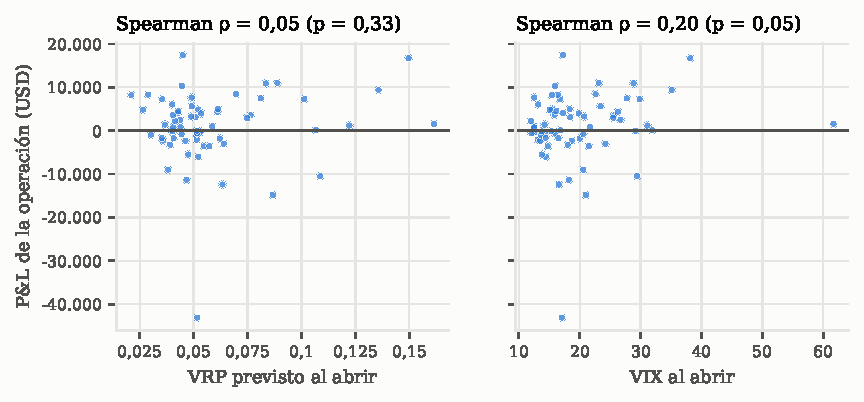
\includegraphics[width=\linewidth]{fig05_trade_level.pdf}
\caption{Resultado de cada una de las 64 operaciones de la venta incondicional frente a la prima prevista y al VIX en la fecha de apertura.}\label{fig:trades}
\end{figure}

\subsection{La comparación con la regla sistemática, revisada}\label{sec:correccion}

La versión original concluía que el modelo aportaba un valor añadido tangible sobre una regla sistemática basada en la prima ingenua: un rendimiento acumulado del 5,95~\% frente al 3,89~\%, con menor riesgo y mayor selectividad (64 operaciones frente a 76). La tabla~\ref{tab:correccion} reproduce esos resultados exactamente y muestra por qué la conclusión no se sostiene.

\begin{table}[!htbp]
\centering
\caption{Comparación de la versión original, revisada (configuración de la tesis, 29/04/2019--31/12/2025)}\label{tab:correccion}
\small
\begin{tabular}{@{}lcccc@{}}
\toprule
& ML (tesis) & Vender siempre & \makecell{Sistemática\\(desde 2018)} & \makecell{Sistemática\\(desde la ventana)} \\
\midrule
Rendimiento total (\%) & 5,95 & 5,95 & 3,89 & 3,92 \\
CAGR (\%) & 0,87 & 0,87 & 0,57 & 0,58 \\
Volatilidad anual (\%) & 2,49 & 2,49 & 2,54 & 2,46 \\
Sharpe (rf 2~\%) & $-0{,}44$ & $-0{,}44$ & $-0{,}55$ & $-0{,}57$ \\
Máxima caída (\%) & $-5{,}23$ & $-5{,}23$ & $-6{,}13$ & $-5{,}93$ \\
CVaR 95~\% diario (\%) & 0,45 & 0,45 & 0,46 & 0,44 \\
Operaciones en la ventana & 64 & 64 & 62 (76) & 63 \\
\bottomrule
\end{tabular}
\par\smallskip\raggedright\footnotesize Entre paréntesis, la cifra de la versión original, que incluía 14 operaciones abiertas entre enero de 2018 y abril de 2019.
\end{table}

La comparación no era homogénea por dos motivos. En primer lugar, como todas las predicciones son positivas y el umbral de entrada es cero, la estrategia guiada por el modelo vende cada vez que no tiene posición: su simulación coincide sesión a sesión con la de vender siempre (primera y segunda columnas), y el modelo no interviene en ninguna decisión. En segundo lugar, la estrategia sistemática se simulaba desde enero de 2018, porque su señal está disponible desde el principio, y su curva se recortaba después a la ventana de evaluación; el recuento de operaciones, en cambio, no se recortaba. Dentro de la ventana, la regla sistemática abre 62 operaciones, no 76, y es ella la que se abstiene en ocasiones, porque su señal es negativa el 6,4~\% de los días. La diferencia de rendimiento procede de esas abstenciones y de que la regla llega a la ventana con una posición abierta; si se inicia el mismo día que la estrategia predictiva, el resultado apenas cambia (3,92~\%). La figura~\ref{fig:correccion} muestra las tres curvas.

\begin{figure}[!htbp]
\centering
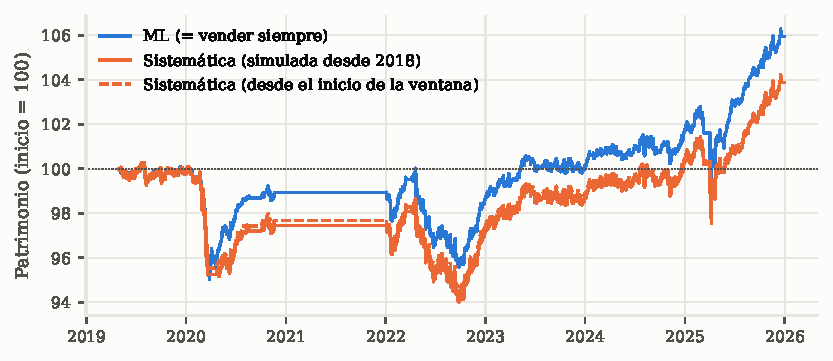
\includegraphics[width=\linewidth]{fig06_corrected_comparison.pdf}
\caption{Patrimonio de la estrategia guiada por el modelo, idéntica a vender siempre, y de la regla sistemática, simulada desde 2018 o desde el inicio de la ventana de evaluación.}\label{fig:correccion}
\end{figure}

La conclusión correcta es que, en esta configuración, el modelo no aporta valor sobre la regla sistemática ni sobre la venta incondicional. El trabajo original sí demostraba que la prima existe y que la cobertura condiciona el resultado; lo que no demostraba es que la señal predictiva mejore la operativa.

\subsection{Costes, colateral y cobertura}\label{sec:costes}

El Sharpe negativo de la versión original merece una precisión. En la simulación, el millón de dólares de capital no devenga intereses, pero el ratio de Sharpe resta un 2~\% anual. Con un tamaño de un contrato, el rendimiento de la estrategia es pequeño frente a ese umbral, y el signo del Sharpe refleja la convención más que la estrategia. La tabla~\ref{tab:costes} y la figura~\ref{fig:steps} descomponen el efecto de cada supuesto sobre la venta incondicional.

\begin{table}[!htbp]
\centering
\caption{Venta incondicional: efecto acumulado de cada supuesto (29/04/2019--31/12/2025)}\label{tab:costes}
\small
\begin{tabular}{@{}lcccc@{}}
\toprule
& \makecell{Tesis (punto\\medio, rf 2~\%)} & \makecell{+ colateral\\al T-Bill 3M} & \makecell{+ venta\\al bid} & \makecell{+ banda\\anidada} \\
\midrule
Rendimiento total (\%) & 5,95 & 26,08 & 24,33 & 11,62 \\
CAGR (\%) & 0,87 & 3,54 & 3,32 & 1,66 \\
Volatilidad anual (\%) & 2,49 & 2,28 & 2,30 & 3,66 \\
Sharpe & $-0{,}44$ & 0,33 & 0,23 & $-0{,}29$ \\
Máxima caída (\%) & $-5{,}23$ & $-4{,}61$ & $-4{,}66$ & $-10{,}45$ \\
\bottomrule
\end{tabular}
\par\smallskip\raggedright\footnotesize Desde la segunda columna, el Sharpe se calcula sobre el exceso frente al T-Bill a tres meses (media del 2,8~\% en la ventana).
\end{table}

\begin{figure}[!htbp]
\centering
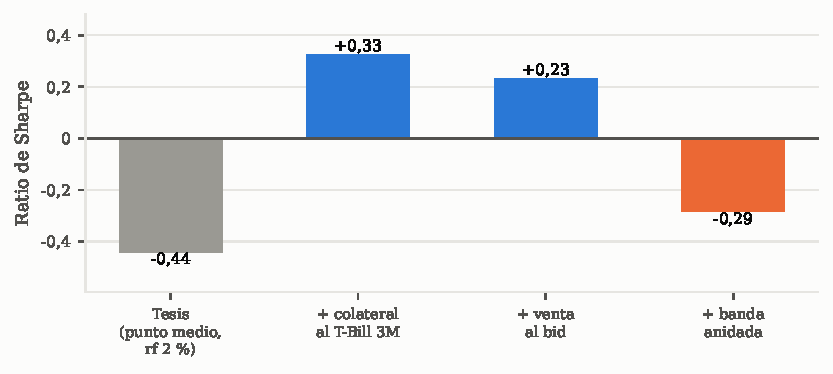
\includegraphics[width=0.85\linewidth]{fig07_sharpe_steps.pdf}
\caption{Ratio de Sharpe de la venta incondicional al añadir cada supuesto.}\label{fig:steps}
\end{figure}

Remunerar el colateral al tipo de la letra del Tesoro, que es lo que ocurre con el margen de una cartera real, y medir el exceso frente a ese tipo eleva el Sharpe de $-0{,}44$ a 0,33. Vender al precio comprador en lugar de al medio cuesta 1,7 puntos de rendimiento acumulado y reduce el Sharpe a 0,23. Con una contabilidad correcta, la venta de volatilidad cubierta obtiene un exceso de rentabilidad positivo, aunque pequeño.

El último paso es el más relevante. La banda de 0,50 se eligió en la versión original como la que maximizaba el rendimiento en la misma muestra evaluada (figura~\ref{fig:band}): una banda estrecha consume la prima en costes (886 rebalanceos con 0,05) y la ausencia de cobertura deja la gamma expuesta (máxima caída del $-15{,}85$~\%). Cuando la banda se elige en cada pliegue con los datos anteriores, la elección salta sin pauta: sin cobertura, 1,00, 0,05, 1,00 y 0,50 (tabla~\ref{tab:band}). El Sharpe cae a $-0{,}29$ y la máxima caída se duplica. La forma de U invertida de la figura~\ref{fig:band} es real en la muestra, pero su máximo no es identificable con antelación.

\begin{figure}[!htbp]
\centering
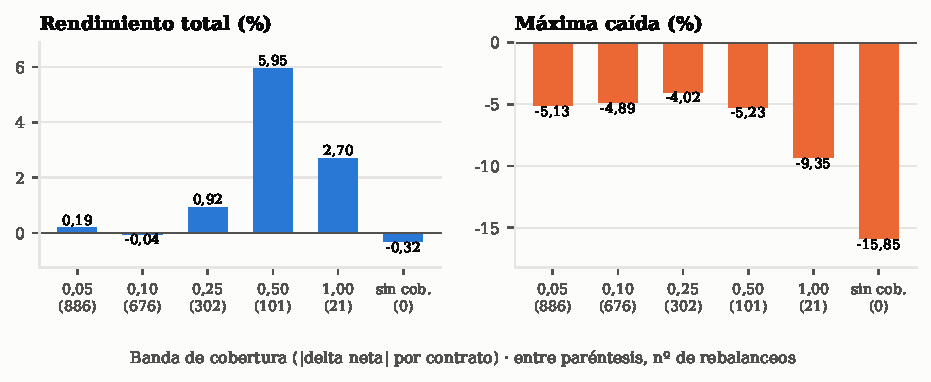
\includegraphics[width=\linewidth]{fig08_hedge_band.pdf}
\caption{Sensibilidad del rendimiento total y de la máxima caída a la banda de cobertura (configuración de la tesis, estrategia guiada por el modelo).}\label{fig:band}
\end{figure}

\begin{table}[!htbp]
\centering
\caption{Elección anidada de la banda: Sharpe de la venta incondicional en los datos anteriores a cada pliegue}\label{tab:band}
\small
\begin{tabular}{@{}lcccccc|c@{}}
\toprule
Pliegue (datos hasta) & 0,05 & 0,10 & 0,25 & 0,50 & 1,00 & Sin cob. & Elegida \\
\midrule
1 (20/03/2019) & $-1{,}54$ & $-1{,}51$ & $-1{,}72$ & $-1{,}91$ & $-1{,}41$ & $\mathbf{-1{,}12}$ & Sin cob. \\
2 (13/07/2020) & $-0{,}57$ & $-0{,}75$ & $-0{,}86$ & $-0{,}81$ & $\mathbf{-0{,}52}$ & $-0{,}75$ & 1,00 \\
3 (02/11/2021) & $\mathbf{-0{,}27}$ & $-0{,}40$ & $-0{,}48$ & $-0{,}58$ & $-0{,}36$ & $-0{,}57$ & 0,05 \\
4 (28/02/2023) & $-0{,}59$ & $-0{,}63$ & $-0{,}64$ & $-0{,}39$ & $\mathbf{-0{,}36}$ & $-0{,}54$ & 1,00 \\
5 (24/06/2024) & $-0{,}30$ & $-0{,}31$ & $-0{,}35$ & $\mathbf{-0{,}27}$ & $-0{,}46$ & $-0{,}60$ & 0,50 \\
\bottomrule
\end{tabular}
\par\smallskip\raggedright\footnotesize Todos los periodos de entrenamiento incluyen 2018 y, desde el pliegue 2, marzo de 2020, de ahí los Sharpe negativos.
\end{table}

\subsection{¿Mejora la magnitud de la predicción?}\label{sec:magnitud}

La regla original solo usaba el signo de la predicción. La tabla~\ref{tab:magnitud} evalúa las alternativas que usan su magnitud en la configuración rigurosa, con la banda anidada y con la banda fija de 0,50, y la figura~\ref{fig:honest} muestra las curvas de patrimonio.

\begin{table}[!htbp]
\centering
\caption{Uso de la magnitud de la predicción (configuración rigurosa, 29/04/2019--31/12/2025)}\label{tab:magnitud}
\small
\begin{tabular}{@{}lcccccc@{}}
\toprule
& \makecell{Vender\\siempre} & ML $>0$ & \makecell{ML $>$\\mediana} & \makecell{ML con\\tamaño} & \makecell{Ingenua $>$\\mediana} & \makecell{Buy \&\\Hold} \\
\midrule
\multicolumn{7}{@{}l}{\textit{Banda elegida en cada pliegue (anidada)}} \\
Rendimiento total (\%) & 11,62 & 11,80 & 20,14 & 15,25 & 16,36 & 132,60 \\
Volatilidad anual (\%) & 3,66 & 3,65 & 1,65 & 2,61 & 3,25 & 20,23 \\
Sharpe & $-0{,}29$ & $-0{,}28$ & 0,00 & $-0{,}23$ & $-0{,}13$ & 0,59 \\
Máxima caída (\%) & $-10{,}45$ & $-10{,}53$ & $-2{,}44$ & $-5{,}95$ & $-10{,}35$ & $-33{,}93$ \\
CVaR 95~\% diario (\%) & 0,60 & 0,60 & 0,28 & 0,45 & 0,49 & 3,07 \\
\midrule
\multicolumn{7}{@{}l}{\textit{Banda fija de 0,50}} \\
Rendimiento total (\%) & 24,33 & 24,50 & 23,12 & 23,39 & 25,19 & -- \\
Volatilidad anual (\%) & 2,30 & 2,30 & 1,69 & 2,12 & 1,81 & -- \\
Sharpe & 0,23 & 0,24 & 0,22 & 0,20 & 0,35 & -- \\
Máxima caída (\%) & $-4{,}66$ & $-4{,}65$ & $-3{,}29$ & $-5{,}26$ & $-4{,}33$ & -- \\
CVaR 95~\% diario (\%) & 0,40 & 0,40 & 0,28 & 0,38 & 0,30 & -- \\
\midrule
Operaciones & 64 & 64 & 30 & 64 & 42 & -- \\
\bottomrule
\end{tabular}
\par\smallskip\raggedright\footnotesize ML con tamaño: 0,82 contratos de media. El Sharpe es el exceso sobre el T-Bill a tres meses; el colateral se remunera a ese tipo.
\end{table}

Con la banda anidada, operar solo cuando la prima prevista supera la mediana histórica reduce la volatilidad a menos de la mitad y la máxima caída del $-10{,}5$~\% al $-2{,}4$~\%, y eleva el Sharpe de $-0{,}29$ a 0,00. El resultado es atractivo a primera vista, pero procede sobre todo de operar menos (30 operaciones frente a 64) en una configuración en la que la cobertura está mal calibrada: con la banda fija de 0,50, la misma regla no mejora a la venta incondicional (0,22 frente a 0,23). El tamaño proporcional tampoco mejora en ninguna de las dos configuraciones. La regla ingenua con el mismo umbral obtiene el mejor Sharpe con banda fija (0,35), de modo que, si filtrar por el nivel de la prima tiene algún valor, no requiere un modelo de aprendizaje automático.

\begin{figure}[!htbp]
\centering
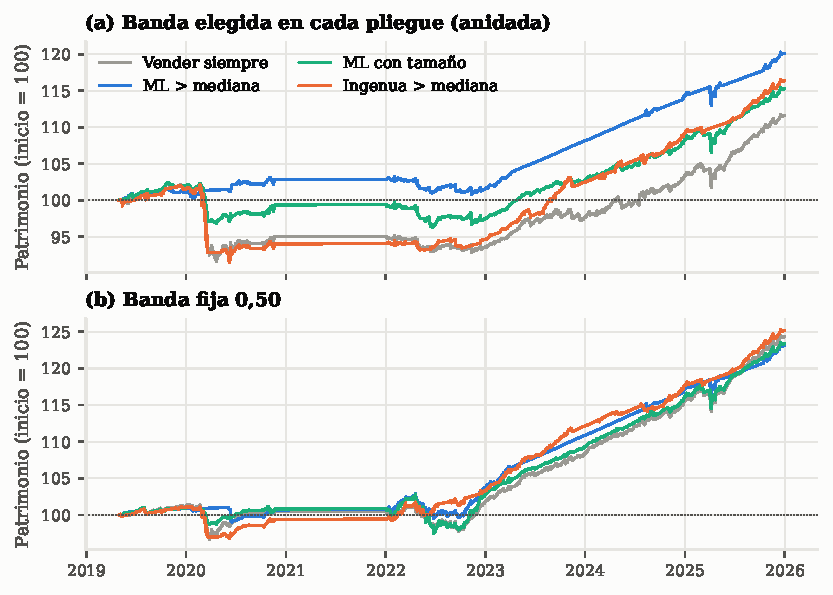
\includegraphics[width=\linewidth]{fig09_honest_equity.pdf}
\caption{Patrimonio de las estrategias en la configuración rigurosa (venta al bid y colateral remunerado), con la banda elegida en cada pliegue y con la banda fija de 0,50.}\label{fig:honest}
\end{figure}

\subsection{La prima en estado puro: swaps de varianza}\label{sec:varswap}

La tabla~\ref{tab:vs} presenta los resultados de la venta mensual de swaps de varianza, promediados sobre los 21 calendarios de entrada posibles, y la figura~\ref{fig:vs} muestra el resultado acumulado y la dispersión entre calendarios.

\begin{table}[!htbp]
\centering
\caption{Swaps de varianza vendidos cada 21 sesiones (media de los 21 calendarios de entrada; P\&L en puntos de volatilidad por unidad de nocional vega)}\label{tab:vs}
\small
\begin{tabular}{@{}lccccc|cc@{}}
\toprule
& & \multicolumn{4}{c|}{Sin límite} & \multicolumn{2}{c}{Límite 2,5$\cdot K$} \\
Estrategia & \makecell{Meses con\\posición} & \makecell{P\&L\\medio} & Sharpe & Asimetría & \makecell{Peor\\mes} & \makecell{P\&L\\medio} & Sharpe \\
\midrule
Incondicional, 2018--2025 & 94,8 & 1,06 & 0,28 & $-6{,}9$ & $-145{,}8$ & 1,97 & 0,71 \\
Incondicional, ventana & 79,0 & 1,22 & 0,31 & $-6{,}8$ & $-145{,}8$ & 2,32 & 0,81 \\
ML $>0$, ventana & 78,4 & 1,19 & 0,31 & $-6{,}7$ & $-145{,}8$ & 2,29 & 0,80 \\
ML $>$ mediana, ventana & 36,0 & 0,31 & 0,50 & $-3{,}5$ & $-96{,}1$ & 1,13 & 0,70 \\
Ingenua $>$ mediana, ventana & 38,6 & 1,03 & 0,71 & $-3{,}9$ & $-77{,}3$ & 1,32 & 0,81 \\
\bottomrule
\end{tabular}
\par\smallskip\raggedright\footnotesize El P\&L medio incluye los meses sin posición (resultado nulo). Sharpe anualizado de los resultados mensuales. Ventana: 29/04/2019--31/12/2025.
\end{table}

\begin{figure}[!htbp]
\centering
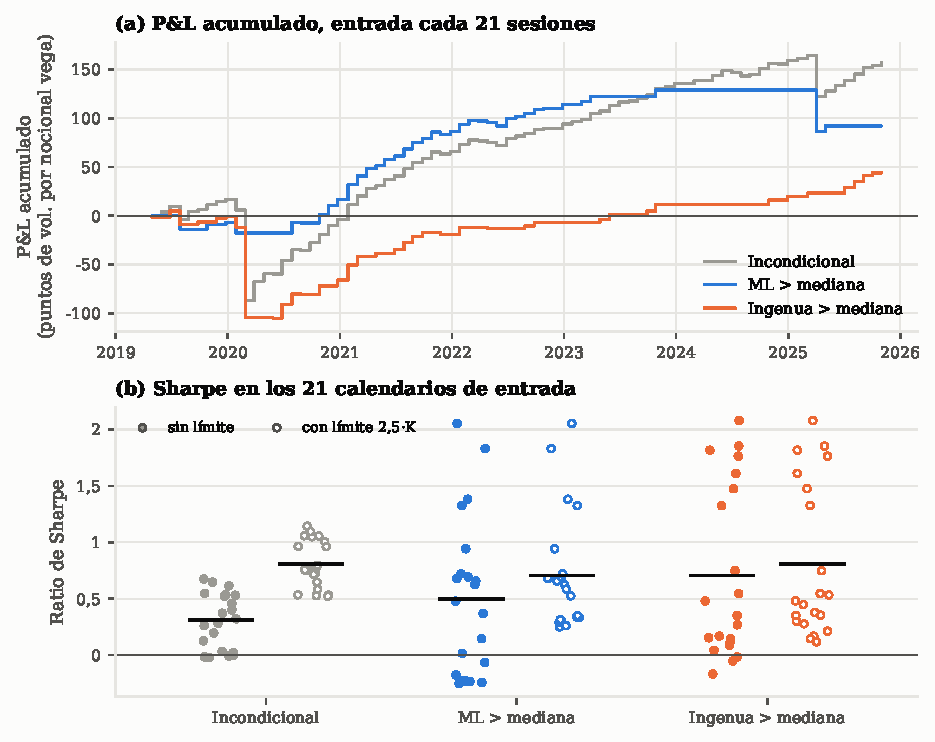
\includegraphics[width=\linewidth]{fig11_varswap.pdf}
\caption{Swaps de varianza vendidos cada 21 sesiones: (a) resultado acumulado con el primer calendario de entrada; (b) Sharpe de cada uno de los 21 calendarios, sin límite y con límite de 2,5$\cdot K$ (las líneas negras son las medias).}\label{fig:vs}
\end{figure}

Los swaps confirman las conclusiones de la estrategia con opciones en un marco que no depende de la ejecución, de la cobertura ni de los datos de opciones. La prima incondicional es positiva en el 81--83~\% de los meses, pero su distribución tiene una asimetría muy negativa ($-6{,}9$), y sin límite un solo mes de 2020 borra años de resultado. Filtrar con la predicción del modelo mejora el Sharpe medio sin límite (0,50 frente a 0,31) a costa de operar menos de la mitad de los meses, pero no con límite (0,70 frente a 0,81). La regla ingenua vuelve a obtener resultados iguales o mejores. Además, la dispersión entre calendarios es enorme: según la fecha de entrada, el Sharpe de la estrategia filtrada por el modelo va de $-0{,}25$ a 2,05. Con unos 80 meses, la fecha de entrada pesa tanto como la señal.

\subsection{Volmageddon}\label{sec:volmageddon}

La figura~\ref{fig:volm} sitúa el episodio de febrero de 2018 en este marco. Esta parte es descriptiva, porque la simulación con opciones empieza en 2019. Durante enero de 2018 el VIX se mantuvo entre 9 y 15 puntos, mientras que, para los swaps vendidos desde el 9 de enero, la volatilidad realizada en las 21 sesiones siguientes fue de 23,5 a 26,4 puntos. Un swap vendido el 22 de enero a un precio de ejercicio de 11,0 realizó 24,8 puntos y perdió 22,3 puntos por unidad de nocional vega, es decir, 2,2 millones de dólares por cada 100.000 dólares de nocional vega, el equivalente a unos 20 meses de prima media (1,06 puntos al mes en 2018--2025). La pérdida no procedió de la sesión del 5 de febrero en sí, sino de haber vendido la volatilidad cuando la implícita era históricamente baja. Una vez producido el salto, la implícita superó a la realizada posterior y los swaps vendidos entre el 5 y el 21 de febrero ganaron entre 3,2 y 12,9 puntos.

\begin{figure}[!htbp]
\centering
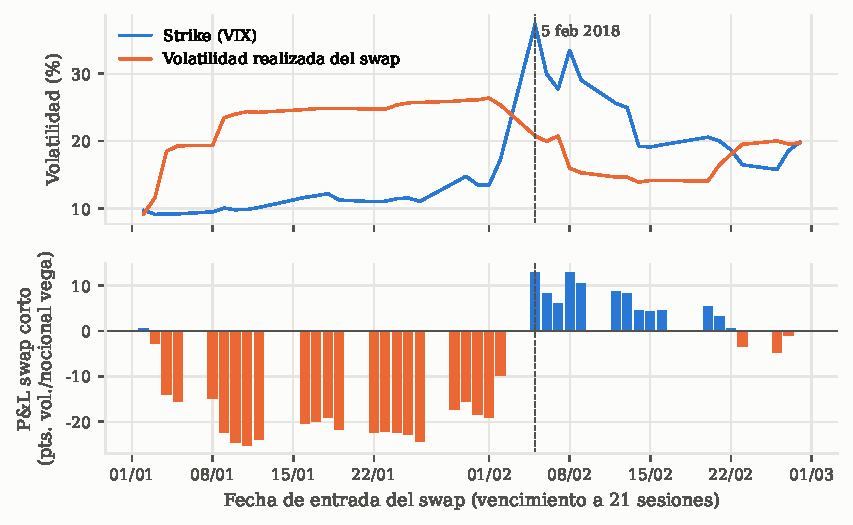
\includegraphics[width=\linewidth]{fig12_volmageddon.pdf}
\caption{Swaps de varianza vendidos entre enero y febrero de 2018: precio de ejercicio (VIX) y volatilidad realizada en las 21 sesiones siguientes (arriba), y resultado por fecha de entrada (abajo). Análisis descriptivo; no forma parte de la simulación con opciones.}\label{fig:volm}
\end{figure}

\subsection{Inferencia}\label{sec:inferencia}

La figura~\ref{fig:boot} y la tabla~\ref{tab:boot} resumen los intervalos de confianza obtenidos por \textit{bootstrap}. Ningún ratio de Sharpe de las estrategias de volatilidad es distinto de cero con un 95~\% de confianza, y ninguna diferencia frente a la venta incondicional es significativa: la mayor, ML $>$ mediana con la banda anidada, tiene un intervalo al 95~\% de $[-0{,}45;\,0{,}95]$. En la muestra disponible no es posible distinguir las variantes entre sí, y cualquier ordenación de la tabla~\ref{tab:magnitud} debe leerse con esa cautela.

\begin{table}[!htbp]
\centering
\caption{Intervalos de confianza por \textit{bootstrap} estacionario (configuración rigurosa, banda anidada; 10.000 remuestreos)}\label{tab:boot}
\footnotesize\setlength{\tabcolsep}{4pt}
\begin{tabular}{@{}lcccc@{}}
\toprule
& Estimación & IC 95~\% & IC 90~\% & P($\leq 0$) \\
\midrule
Sharpe: vender siempre & $-0{,}29$ & $[-0{,}84;\ 0{,}49]$ & $[-0{,}76;\ 0{,}38]$ & 0,76 \\
Sharpe: ML $>$ mediana & 0,00 & $[-0{,}55;\ 0{,}60]$ & $[-0{,}46;\ 0{,}50]$ & 0,49 \\
Sharpe: Buy \& Hold & 0,59 & $[-0{,}03;\ 1{,}35]$ & $[0{,}07;\ 1{,}23]$ & 0,03 \\
Dif.: ML $>0$ $-$ vender siempre & 0,01 & $[-0{,}02;\ 0{,}04]$ & $[-0{,}01;\ 0{,}03]$ & 0,37 \\
Dif.: ML $>$ mediana $-$ vender siempre & 0,29 & $[-0{,}45;\ 0{,}95]$ & $[-0{,}35;\ 0{,}85]$ & 0,26 \\
Dif.: ML con tamaño $-$ vender siempre & 0,06 & $[-0{,}21;\ 0{,}24]$ & $[-0{,}16;\ 0{,}21]$ & 0,36 \\
Dif.: ingenua $>$ mediana $-$ vender siempre & 0,15 & $[-0{,}18;\ 0{,}72]$ & $[-0{,}12;\ 0{,}61]$ & 0,18 \\
Dif. swap: ML $>$ mediana $-$ incond. & 0,09 & $[-1{,}62;\ 1{,}45]$ & $[-1{,}43;\ 1{,}25]$ & 0,53 \\
\bottomrule
\end{tabular}
\end{table}

\begin{figure}[!htbp]
\centering
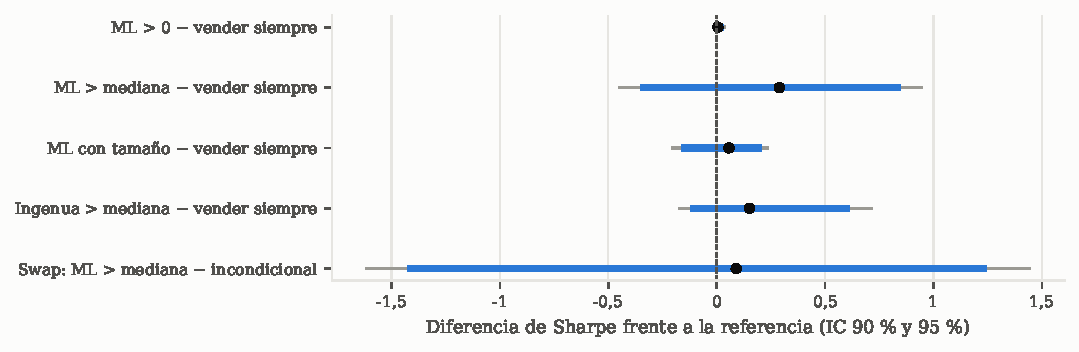
\includegraphics[width=\linewidth]{fig10_bootstrap.pdf}
\caption{Diferencias de Sharpe frente a la referencia, con intervalos de confianza al 90~\% (barra gruesa) y al 95~\% (barra fina).}\label{fig:boot}
\end{figure}

\section{Limitaciones y extensiones}\label{sec:limitaciones}

\paragraph{Valoración al final de la vida de la opción.} La cadena depurada abarca de 15 a 45 días hasta el vencimiento, de modo que los últimos 15 días de cada \textit{straddle}, cuando la gamma es máxima, se valoran con Black-Scholes y la última volatilidad implícita. Es la limitación más relevante para el riesgo de cola, y la única que exige nuevos datos de opciones: una cadena de seguimiento de 0 a 45 días permitiría valorar toda la vida de la posición con precios de mercado.

\paragraph{Año 2021.} La ausencia de cadenas de 2021 elimina el año más favorable para el vendedor de volatilidad (tabla~\ref{tab:vs_year}). El análisis con swaps de varianza lo cubre, pero la estrategia con opciones no.

\paragraph{Supuestos de ejecución.} La venta al precio comprador corrige el diferencial de entrada, pero la cobertura se modela con un deslizamiento de 1 punto básico y sin impacto de mercado, la liquidación se realiza con el cierre del día de vencimiento y no con el precio especial de apertura de las opciones mensuales del SPX, y el tamaño es fijo.

\paragraph{Potencia estadística.} Los resultados descansan sobre una única trayectoria de 6,7 años, 64 operaciones y unos 80 meses, dominada por un mercado alcista. Los intervalos de la sección~\ref{sec:inferencia} muestran que esa muestra no permite distinguir entre las variantes.

\paragraph{Selección del modelo.} La validación anidada elimina el sesgo de selección de los hiperparámetros y de la banda, pero la arquitectura general (variables, horizonte, pérdida, malla) se diseñó con conocimiento de la muestra.

\paragraph{Extensiones.} Las líneas más prometedoras son: (i) una cadena de seguimiento completa y la recuperación de 2021; (ii) predecir directamente el resultado de la operación cubierta, en lugar del diferencial de volatilidades, o reformular el problema como una clasificación de regímenes de prima negativa; (iii) un dimensionamiento orientado a un objetivo de volatilidad que use la predicción del riesgo, no de la prima; (iv) extender la muestra hacia atrás e incluir opciones semanales (SPXW) para aumentar el número de operaciones independientes; y (v) contrastar las reglas con varios activos (VIX, futuros sobre el VIX, otros índices).

\section{Conclusiones}\label{sec:conclusiones}

La prima de riesgo de varianza del S\&P~500 es persistente y puede capturarse: con una contabilidad correcta del colateral y venta al precio comprador, la venta sistemática de \textit{straddles} cubiertos obtiene un exceso de rentabilidad positivo con una fracción del riesgo de la renta variable. La predicción de la prima con \textit{gradient boosting} mejora en promedio a las referencias ingenuas, aunque de forma modesta, inestable entre periodos y no significativa en error cuadrático. Esa información no se traslada a la operativa: el modelo predice una prima positiva en todas las sesiones, su predicción no ordena el resultado de las operaciones, y las reglas que usan su magnitud no mejoran de forma significativa a la venta incondicional ni a una regla ingenua.

El resultado económico lo determina la gestión del riesgo. La banda de cobertura explica más variación del resultado que cualquier señal, y su óptimo en la muestra no es identificable con antelación. Para un vendedor de volatilidad, la pregunta relevante no es cuánto valdrá la prima el mes próximo, cuyo nivel típico se conoce bien, sino cuándo puede volverse muy negativa y cuánto cuesta protegerse de ello. Ese es el problema que una siguiente versión de este sistema debería abordar.

\FloatBarrier
\bibliographystyle{../plainnat-es}
\bibliography{../refs}

\clearpage
\appendix
\section{Hiperparámetros}\label{app:hiper}

\begin{table}[!htbp]
\centering
\caption{Malla de búsqueda (40 combinaciones aleatorias con semilla 42) y elección por pliegue}\label{tab:hiper}
\small
\begin{tabularx}{\linewidth}{@{}lX@{}}
\toprule
Parámetro & Valores \\
\midrule
Tasa de aprendizaje & 0,01; 0,05; 0,1 \\
Hojas (LightGBM) & 31; 63; 127 \\
Profundidad (XGBoost) & 3; 5; 7 \\
Submuestreo de filas y de columnas & 0,7; 0,8; 0,9 \\
Regularización L1 y L2 & 0; 0,1; 1; 10 \\
Árboles; umbral de Huber & 400; $\delta=0{,}02$ \\
\midrule
Tesis (XGBoost) & tasa 0,1; profundidad 3; submuestreo 0,9 y 0,9; L1 1; L2 0,1 \\
Anidada, pliegue 1 & LightGBM: tasa 0,1; 63 hojas; 0,8 y 0,8; L1 1; L2 10 \\
Anidada, pliegues 2--5 & XGBoost: profundidad 3, 5, 7 y 3; el resto, como en la tesis salvo L2 1 (pliegue 3) y L1 0,1 (pliegue 4) \\
\bottomrule
\end{tabularx}
\end{table}

\section{Reproducibilidad}

El código, organizado como un paquete de Python, está disponible en \repourl. El fichero \texttt{scripts/run\_pipeline.py} reproduce los resultados de la versión original y \texttt{scripts/run\_extensions.py}, los de esta revisión. Los datos de ThetaData no pueden redistribuirse; el repositorio incluye el script de descarga, las predicciones fuera de muestra de la versión original y todas las tablas de resultados. Las semillas son fijas (42). XGBoost no produce predicciones idénticas bit a bit entre plataformas: al reentrenar en Linux, el RMSE por pliegue varía hasta 0,003 respecto a la ejecución original, aunque todas las predicciones siguen siendo positivas y la simulación no cambia.

\end{document}
